\section{Existing Games}

Games using procedural content generation is far from new. The first game featuring this concept was the game Elite from 1984\cite{firstpcg}. However over the last few years the concept have been used more. A lot of new games, and especially indie games, seems to take advantage of procedural content generation.

We will in this section take a look at a few games that uses procedural content generation and look into what these games are all about to get an understanding on what is on the game market.


\subsection{Minecraft}

When talking about procedural content generation one of the first game titles that may come to mind is Minecraft. Minecraft is originally made by "Notch" (Markus Persson), and later on managed by "Jeb" (Jens Bergensten)\cite{Minecraft} and recently bought by Microsoft. Minecraft is a sandbox, survival, crafting game and the game makes it possible for players to, not only walk around and explore the world, but also manipulate and create complex structures as seen in \figref{fig:MinecraftCity} as well as replicates of real buildings. Since Minecraft is a sandbox game this means there is no real objectives for the player to accomplish, but the player(s) can makes their own to complete, eg. build a house. This makes it possible for the player to replay the game with new objectives each time the game is played.

\begin{figure}[H]
	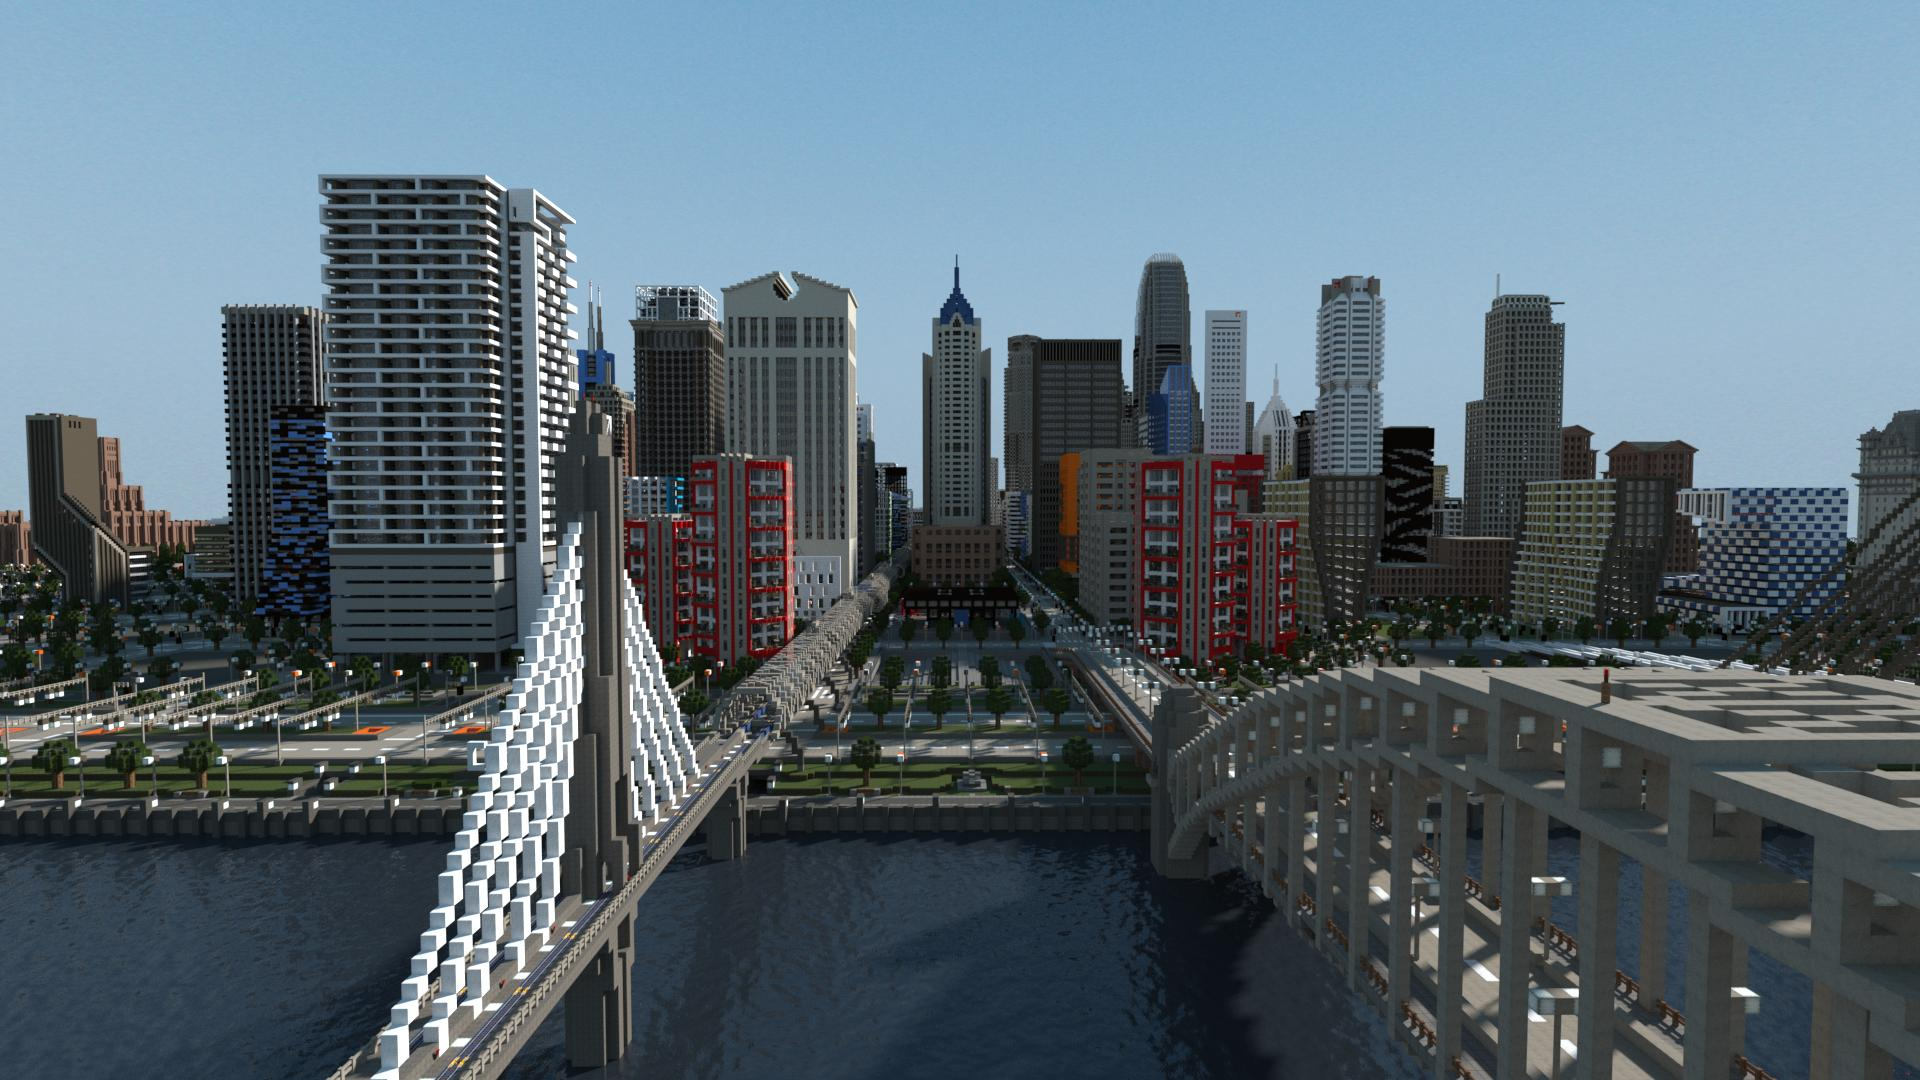
\includegraphics[width=0.7\linewidth]{img/MinecraftCity}
	\centering
	\caption{The image shows a city built in minecraft}
	\label{fig:MinecraftCity}
\end{figure}


\subsection{Terraria}

Terraria\cite{Terraria} is yet another game that have many similarities to Minecraft. Terraria is a 2D side scrolling game as seen in \figref{fig:Terraria} and have been called the 2D version of Minecraft by many people. The biggest difference is that Terraria does provide the player with some task that at some point in the game should be completed to be able to move on to other challenges. The way of adding task to a sandbox game seems like a great idea as it makes sure that the player have some sort of guideline to how they need to play the game, and most do certain things before unlocking new content.

\begin{figure}[H]
	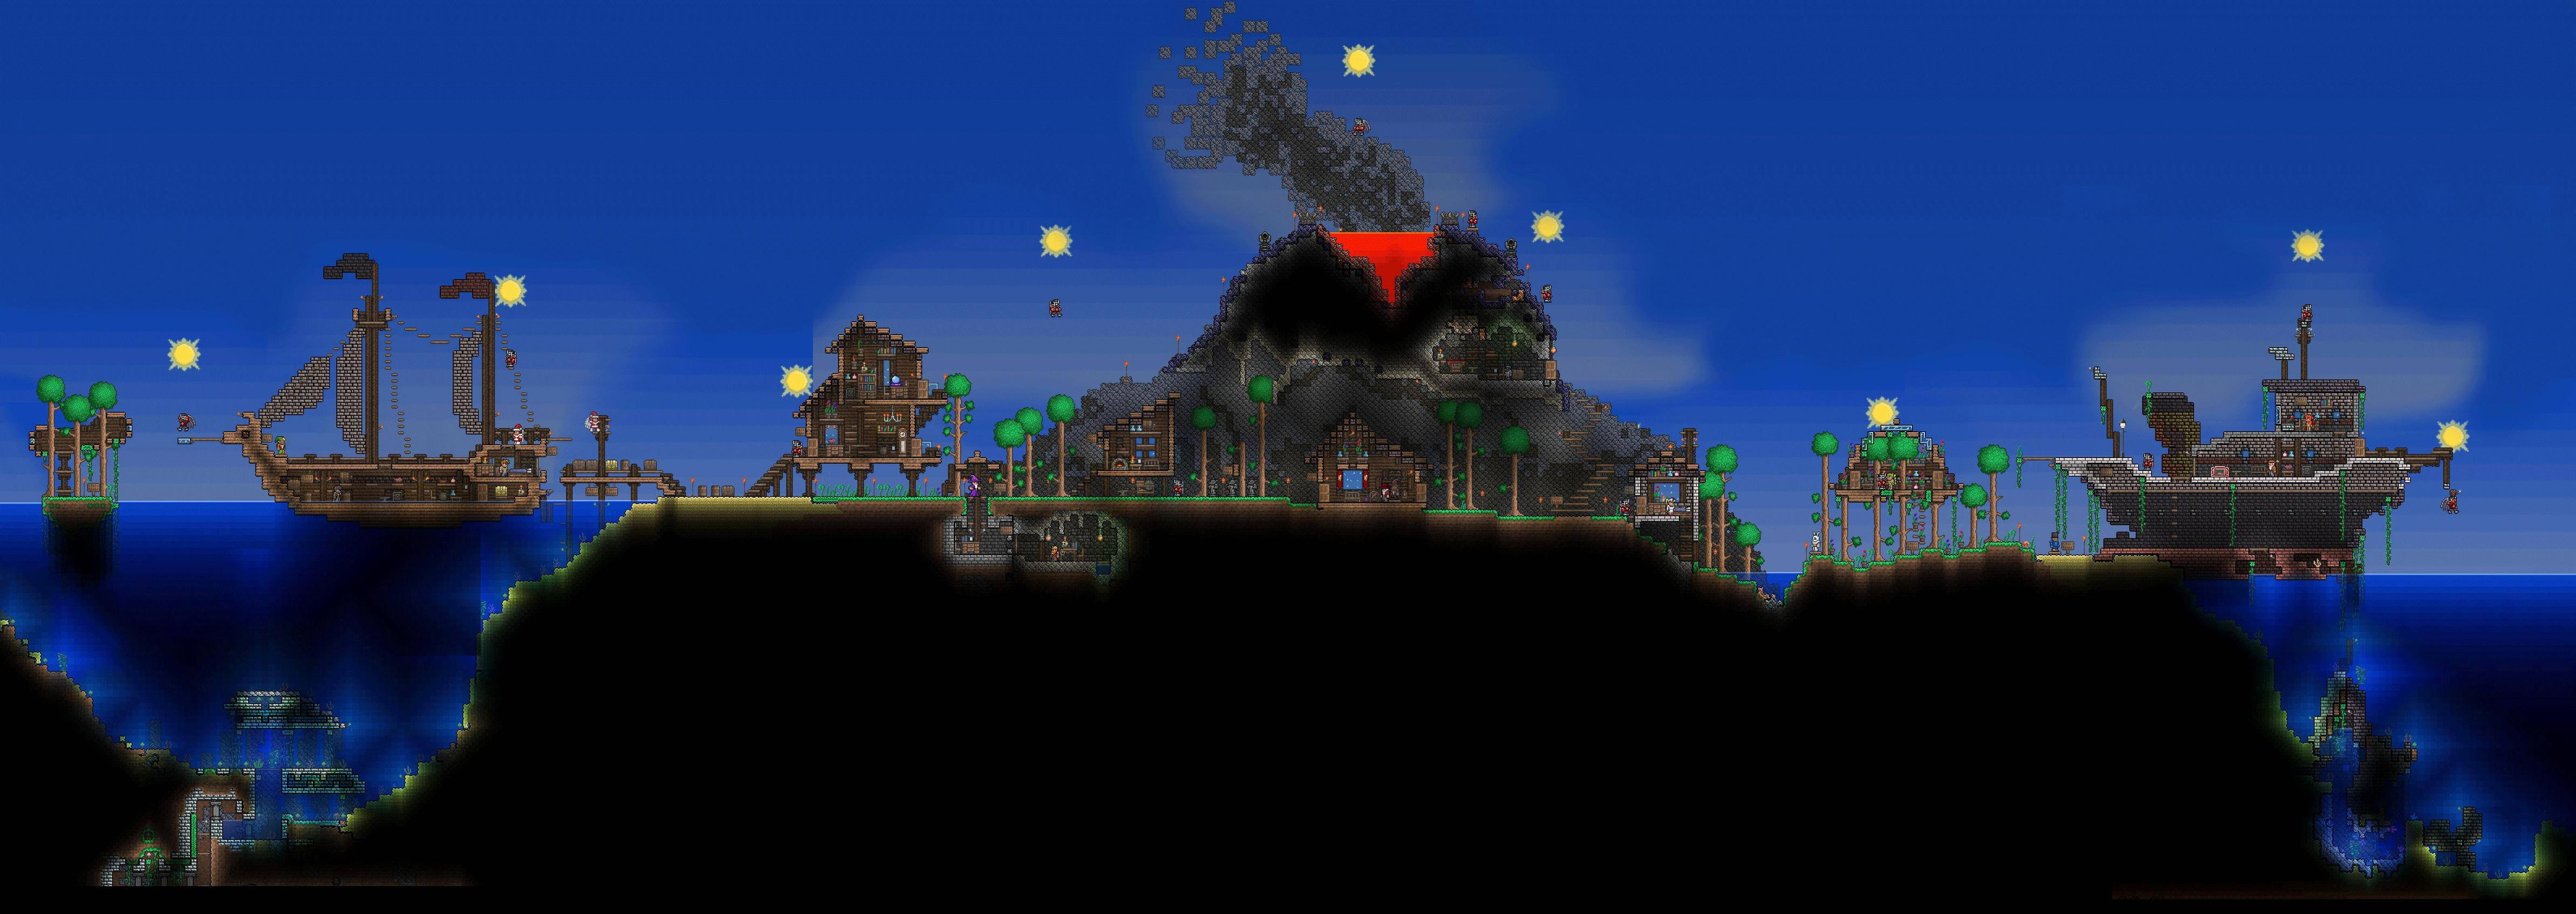
\includegraphics[width=0.7\linewidth]{img/Terraria}
	\centering
	\caption{The image is a from Terraria of a volcanic island. The image is cut together from multiple images.}
	\label{fig:Terraria}
\end{figure}


\subsection{Rust}

A newer game on the market is Rust\cite{Rust}. Rust have moved away from the blocks Minecraft and Terraria is using and have as seen in\figref{fig:Rust} smooth terrain which at some places could look like a wilderness found on earth. The game is as both Minecraft and Terraria a crafting survival game, but rust does set focus on first person shooter a lot. The main objective is to find material to survive and make unfriendly players keep their distance as death results in a reset of your character.

\begin{figure}[H]
	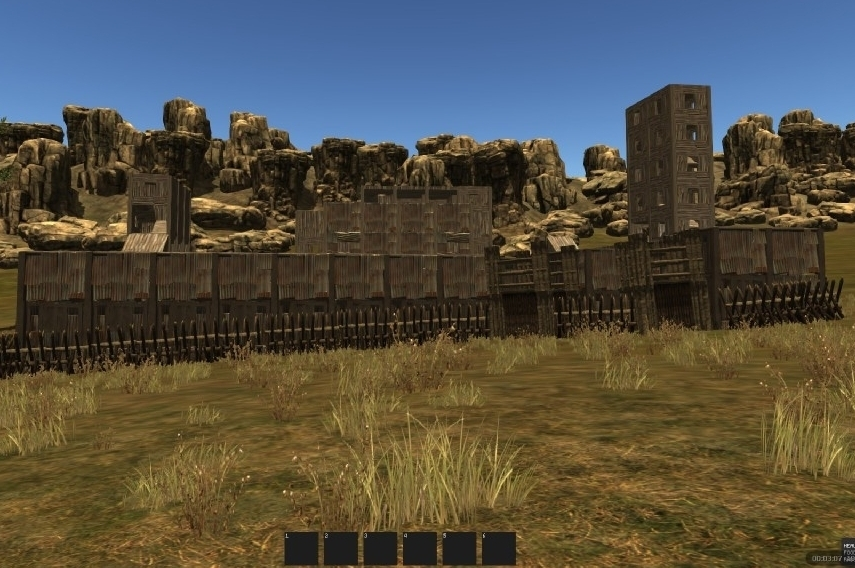
\includegraphics[width=0.7\linewidth]{img/Rust}
	\centering
	\caption{The image shows a highly secured fortress built in Rust}
	\label{fig:Rust}
\end{figure}


\subsection{SpeedTree}

SpeedTree\cite{SpeedTree} is a program that does one thing only, but does it very well; creating trees, as seen in \figref{fig:SpeedTree}. It's far from a game but it does use procedural content generation to generate highly detailed 3D meshes for trees. SpeedTree is used in many triple A games, and animation films. This shows us that procedural content generation not only used in games but have great potentials for being used for other purposes.

\begin{figure}[H]
	\includegraphics[width=0.7\linewidth]{img/SpeedTree}
	\centering
	\caption{A basic tree created with SpeedTree}
	\label{fig:SpeedTree}
\end{figure}


\section{Thoughts about the Game Market}

After looking at a bunch of games it seems that a lot of these have a common theme of crafting, adventure and survival. It makes one wonder if it could be possible to break the boundaries and try some others and new themes that could work well with procedural content generation. There have also been other themed games such as real time strategy such as the game Empire Earth, but the game market right now seem to have the same common themes in procedural content generation games. It may be limited what is possible to accomplish in the timespan of this project, but our goal is to have a fully working world.